\documentclass[border=0.125cm]{standalone}
\usepackage{tikz}
\usepackage{pgfplots}
\usepackage{graphicx}

\usetikzlibrary{decorations.pathmorphing}
\pgfplotsset{compat=newest}
\usetikzlibrary{shapes.geometric,arrows,fit,matrix,positioning}
\tikzset{main node/.style={circle,fill=black!20,draw,minimum size=3.5mm,inner sep=0pt},
         every node/.style={circle,fill=black,draw,minimum size=1mm,inner sep=0pt,label distance=-1mm},
         subtree/.style={isosceles triangle,fill=blue!20,draw,minimum size=4mm,inner sep=0pt,shape border rotate=90},
         edge label/.style = {rectangle,draw=none,fill=none}
}
\begin{document}
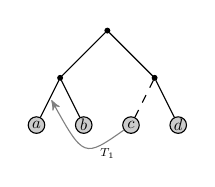
\begin{tikzpicture}[-,>=stealth', 
level 1/.style={sibling distance = 20mm},
level distance = 1cm, 
scale=0.6,
transform shape]
\node (0) {}
    child{
        [sibling distance = 10mm] node (1) {}
            child{
                node [main node] (2) {$a$}
            }
            child{
                node [main node] (3) {$b$}
            }
    }
    child{
        [sibling distance = 10mm] node (4) {}
            child[edge from parent path = {(\tikzparentnode ) -- (\tikzchildnode) [dashed]}]{
                node [main node] (5) {$c$}
            }
            child{
                node [main node] (6) {$d$}
            }
    }
;


\node [edge label, xshift = 0mm, below=25mm, align=flush center] at (0){
        \scriptsize{$T_1$}};
\node[edge label,above right = 4mm and 1mm of 2] (final) {};        
\draw[->,gray] (5) .. controls (-5mm,-27mm) .. (final);
\end{tikzpicture}

\begin{tikzpicture}[->]
\node[edge label] (0) {};
\node [edge label, above=10mm, align=flush center] (a) at (0){};
\node [edge label, xshift = 5mm, above=10mm, align=flush center] (b) at (0){};
\draw (a) -- (b) node[edge label,left] {};        
\end{tikzpicture}

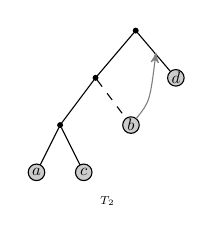
\begin{tikzpicture}[-,>=stealth', 
level 1/.style={sibling distance = 17mm},
level distance = 1cm, 
scale=0.6,
transform shape]
\node (0) {}
    child{
        [sibling distance = 15mm] node (1) {}
            child{
                [sibling distance = 10mm] node (2) {}
                    child{
                        node [main node] (3) {$a$}
                    }
                    child{
                        node [main node] (4) {$c$}
                    }
            }
            child[edge from parent path = {(\tikzparentnode ) -- (\tikzchildnode) [dashed]}]{
                node [main node] (5) {$b$}
            }
    }
    child{
        node [main node] (6) {$d$}
    }
;
\node [edge label, xshift = -6mm, below=35mm, align=flush center] at (0){
        \scriptsize{$T_2$}};
\node[edge label,above right = 4mm and -6mm of 6] (final) {};        
\draw[->,gray] (5) .. controls (3mm,-15mm) .. (final);        
\end{tikzpicture}

\begin{tikzpicture}[->]
\node[edge label] (0) {};
\node [edge label, above=10mm, align=flush center] (a) at (0){};
\node [edge label, xshift = 5mm, above=10mm, align=flush center] (b) at (0){};
\draw (a) -- (b) node[edge label,left] {};        
\end{tikzpicture}

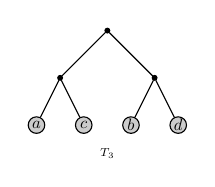
\begin{tikzpicture}[-,>=stealth', 
level 1/.style={sibling distance = 20mm},
level distance = 1cm, 
scale=0.6,
transform shape]
\node (0) {}
    child{
        [sibling distance = 10mm] node (1) {}
            child{
                node [main node] (2) {$a$}
            }
            child{
                node [main node] (3) {$c$}
            }
    }
    child{
        [sibling distance = 10mm] node (4) {}
            child{
                node [main node] (5) {$b$}
            }
            child{
                node [main node] (6) {$d$}
            }
    }
;
\node [edge label,xshift = 0mm , below=25mm, align=flush center] at (0){
        \scriptsize{$T_3$}};
\end{tikzpicture}
\end{document}






